%\documentclass[brudnopis]{xmgr}
% Jeśli nowe rozdziały mają się zaczynać na stronach
% nieparzystych:
\documentclass[openright]{xmgr}

%\defaultfontfeatures{Scale=MatchLowercase}
%\setmainfont[Numbers=OldStyle,Ligatures=TeX]{Minion Pro}
%\setsansfont[Numbers=OldStyle,Ligatures=TeX]{Myriad Pro}
% for fontspec version < 2.0
\setmainfont[Numbers=OldStyle,Mapping=tex-text]{Minion Pro}
\setsansfont[Numbers=OldStyle,Mapping=tex-text]{Myriad Pro}
%\setmonofont[Scale=0.75]{Monaco}

% Opcjonalnie identyfikator dokumentu
% drukowany tylko z włączoną opcją 'brudnopis':
\wersja   {wersja wstępna [\ymdtoday]}

\author   {Kamil Pek}
\nralbumu {231\,050}
\email    {kpek@sigma.ug.edu.pl}

\title    {TrainCMS --- System zarządzania treścią witryny internetowej}
\date     {2017}
\miejsce  {Gdańsk}

\opiekun  {dr W. Bzyl}

% dodatkowe polecenia
%\renewcommand{\filename}[1]{\texttt{#1}}
%\definecolor{stress}{cmyk}{0,1,0.13,0} % RubineRed
%\definecolor{topic}{cmyk}{0.98,0.13,0,0.43} % MidnightBlue

\usepackage{listings}
\renewcommand{\lstlistingname}{kodów źródłowych}
\renewcommand{\lstlistlistingname}{Spis \lstlistingname}

\begin{document}

% streszczenie
\begin{abstract}
W pracy przedstawiono wersję beta systemu zarządzania treścią witryny internetowej „TrainCMS”. W trakcie pracy zaimplementowano publikowanie artykułów, kategoryzację, wyświetlanie listy kategorii na pasku nawigacji. Stworzono User Interface, który wyświetla wszystkie artykuły na stronie głównej, niezależnie od kategorii w kolejności malejącej od daty dodania oraz kalendarz wydarzeń. Do artykułów i wydarzeń w kalendarzu zaimplementowano możliwość załączania ilustracji oraz dodawania komentarzy.

Zaimplementowano panel administratora do zarządzania artykułami, kategoriami, komentarzami, tagami, użytkownikami i kalendarzem oraz do podglądu statystyk.

Do implementacji użyto technologie takie jak Ruby, Ruby on Rails, ZURB Foundation, jQuery Turbolinks, Plataformatec Devise, CarrierWave, RMagick, reCAPTCHA, CKEditor, Chartkick, Prawn.
\end{abstract}

% słowa kluczowe
\keywords{cms, ruby on rails, calendar, comments, tags}

% tytuł i spis treści
\maketitle

% wstęp
\introduction
Podczas kilkuletniej pracy z najpopularniejszymi aplikacjami w tej kategorii, takimi jak Joomla i WordPress nabyłem doświadczenie oraz swój pogląd na to jak ma wyglądać system zarządzania treścią (ang. Content Managment System, CMS). Naturalnym stało się więc stworzenie własnego systemu, przy okazji prezentując jak najszerszą część umiejętności nabytych w trakcie trwania studiów.

Istniejące systemy są często wybierane przez między innymi lokalne serwisy informacyjne, przedsiębiorstwa i instytucje, dlatego w swoim systemie zawarłem funkcjonalności, które na pewno przydadzą się różnym podmiotom w skutecznym zaistnieniu w Internecie.

Podczas tworzenia interfejsu użytkownika i administratora, kierowałem się głównie ergonomią użytkowania i przedstawieniem możliwości jakie prezentuje system w jak najbardziej przystępny sposób tak, aby początkujący użytkownik mógł poruszać się w sposób intuicyjny po aplikacji.

\chapter{Wstęp i opis problemu}

\section{Porównanie dostępnych rozwiązań z systemem TrainCMS}

Na rynku systemów zarządzania treścią znajdziemy sporo różnych rozwiązań. W~dalszej części rozdziału przybliżę dwa najbardziej popularne produkty, będzie to Joomla i WordPress\footnote{Istnieje jeszcze jeden bardzo popularny system zarządzania treścią - Drupal. Podobnie jak oba opisane wyżej systemy, wyprodukowany został w technologii języka PHP i jest udostępniony na otwartej licencji.}. Systemy różnią się od siebie pod wieloma względami. Rozwiązanie przedstawione przeze mnie jakim jest TrainCMS różni się  przede wszystkim technologią wykonania, gdyż oba wcześniej wymienione systemy wyprodukowane są technologii języka PHP i bazy danych MySQL, gdzie mój system opiera się na frameworku Ruby On Rails i bazie danych PostgreSQL.

\subsection{Joomla!}

Joomla jest to system zarządzania treścią, napisany w języku PHP, wykorzystujący do swojego działania system zarządzania bazą danych MySQL, rozpowszechniany na licencji GPL i jest dostępny bezpłatnie. Nazwa Joomla w języku suahili oznacza razem.   
System ten oferuję obsługę wielu kont użytkownika, wyszukiwarkę zaimplementowaną w User Interface, tworzenie wydruków artykułów, dołączanie ilustracji do artykułu, komentowanie artykułów przez niezalogowanych użytkowników. Wymienione funkcjonalności pokrywają się z możliwościami stworzonego przeze mnie systemu. 

TrainCMS posiada także inne możliwości, których nie oferuję Joomla w wersji podstawowej, jest to kalendarz wydarzeń, dodawanie załączników, generowanie dokumentów pdf zawierających artykuły, przedstawienie statystyk w formie graficznej, karuzela ilustracji wyróżnionych artykułów. Natomiast niektóre z rozwiązań zostały rozszerzone względem Joomli są to komentarze, które w projekcie TrainCMS rejestrują adres IP komentującego. 

Znajdziemy także w Joomli takie funkcję, których nie posiada mój system. Jednym z takich rozwiązań jest tworzenie zagnieżdżonej struktury menu w formie drzewiastej. Kolejnym rozwiązaniem jest możliwość zmiany szablonu frontu strony i szablonu zaplecza witryny. Główną funkcjonalnością Joomli jest możliwość łatwego rozszerzania możliwości strony za pomocą pluginów i komponentów. Podczas porównywania obu systemów należy pamiętać, że Joomla jest produktem z wieloletnim doświadczeniem na rynku, tworzonym przez zespół programistów z całego świata. Rozwiązania oparte na Joomli znajdują zastosowanie głównie przy dużych witrynach.

\subsection{WordPress}

WordPress jest systemem zarządzania treścią napisanym w języku PHP, wykorzystujący systemem zarządzania bazą danych MySQL i jest dystrybuowany na licencji GPL i dostępny bezpłatnie. 

System WordPress jest zdecydowanie mniej rozbudowany w porównaniu do Joomli. Oferuje on takie funkcjonalności jak podstawową kategoryzację, tagowanie i komentowanie artykułów, obsługę wielu kont użytkownika, odrębny interfejs dla użytkownika gościa, zwykłego użytkownika i administratora oraz podgląd statystyk jest również w pełny responsywny. Wszystkie wymienione funkcjonalności pokrywają się z zaimplementowanymi w systemie TrainCMS.

W TrainCMS znajdziemy także inne możliwości, których nie oferuję WordPress w wersji podstawowej, jest to kalendarz wydarzeń, dodawanie załączników, generowanie dokumentów pdf zawierających artykuły oraz karuzela ilustracji wyróżnionych artykułów. Natomiast niektóre z rozwiązań zostały rozszerzone względem Joomli są to komentarze, które w projekcie TrainCMS rejestrują adres IP komentującego. 

Należy w tym miejscu wspomnieć, że główną funkcjonalnością WordPress jest łatwość instalacji i zmiany wielu dostępnych szablonów strony. WordPress jest produktem z utartą pozycja na rynku systemów zarządzania treścią, który podobnie jak Joomla jest tworzony przez zespół programistów z całego świata. Witryny obsługiwane przez WordPress to głównie blogi.

\newpage

\section{Możliwości zastosowania praktycznego}

System TrainCMS został opracowany w taki sposób, aby sprostać wielu wymaganiom różnych użytkowników. Oferuje sporo możliwości, które przypadną do gustu każdemu i będą zarazem bardzo przydatne w codziennej pracy nad własna witryną Internetową. Reasumując możliwości serwisu ogranicza jedynie wyobraźnia administratora.

\subsection{Strona wizytkówa}

W celu stworzenia optymalnej i efektownej strony wizytówki należałoby uruchomić tryb statycznej strony głównej. W tymże celu utworzymy zakładkę, którą oznaczymy jako strona główna. Ilość pozostałych zakładek jest dowolna. Może się też zdarzyć potrzeba prowadzenia minibloga lub prostych aktualności firmy, tutaj posłużymy się kategoriami i artykułami. Łącza do kategorii będą wyswietlona na górnym pasku nawigacji co ułatwi poruszanie się po stronie.  Po odpowiednim według operatora strony rozmieszczeniu informacji, możemy przejść do podglądu statystyk, które w tym przypadku mogą wyświetlić informację na przykład o tym, która sekcji informacji jest najbardziej popularna. 

\subsection{Internetowe portfolio}

Każda osoba tworząca w Internecie portfolio swojej działalności zamierza przyciągnąć w ten sposób jak największą liczbę nowy klientów. Aby skutecznie rozwiązać ten problem należy każde dzieło zaprezentować w osobnym artykule. Natomiast informacje, które klient chciałby, aby były zawsze łatwo dostępne, powinno sie umieścić w przygotowanych do tego zakładkach, do których to łącza będą wyswietlane na górnym pasku nawigacji. Można też przyjąć inne podejście do tego tematu, otóż ustawić stronę główna jako stronę statyczną, następnie utworzyć kategorię, do której łącze podobnie jak do zakładek ukaże się na górnym pasku nawigacji, w której to umiścimy dzieła swojej działalności. 

\subsection{Serwis informacyjny}

W tym rozwiązaniu znajdą zastosowanie wszystkie zaimplementowane w systemie funkcjonalności. Większość rozwiązań została wyprofilowana właśnie na tego typu zastosowania. Głównym szkieletem w tym przypadku będzie możliwość tworzenia wielu kategorii, gdzie redaktor takiego serwisu będzie mógł z pełną łatwością organizować wszystkie tematy poruszane na portalu i jednocześnie wszystkie artykuły z każdej kategorii będą wyświetlane na stronie głównej. Gorące tematy będzie można oznaczać jako wyróżnione i tym sposobem będą przez cały widoczne na szczycie karuzeli. Gość odwiedzający serwis z łatwością wejdzie w interakcję ze stroną poprzez system komentarzy, operator serwisu będzie mógł korzystać z przejrzystych statystyk i za ich pomocą wyciągać wnioski na temat pracy portalu i planować dalszy jego rozwój. Z pomocą dla nowych gości przyjdą tagi, dzięki którym będzie można szybko wyszukać artykuły poruszające dany temat. Łatwiejsze stanie się planowanie różnego rodzaju imprez za pomocą wbudowanego kalendarza wydarzeń. Autor piszący artykuły dla serwisu nie będzie musiał zagłębiać się w panel zaplecza, na stronie głównej po zalogowaniu znajdzie skróty do najważniejszych funkcji takich jak nowy artykuł, lista własnych artykułów oraz lista komentarzy pod tymi artykułami. Jeżeli autor zeche to ma możlwiość wyłączenia komentarzy. Jeżeli nadejdzie taka potrzeba, mozęmy skorzystać z zaimplemenotwanego mechanizmu zakładek, które to po utworzeniu wyśweitlane będą na górnym pasku nawigacji.

\chapter{Projekt i analiza}

\newpage

\section{Diagram związków encji}

\begin{figure}[!tbh]
\centering
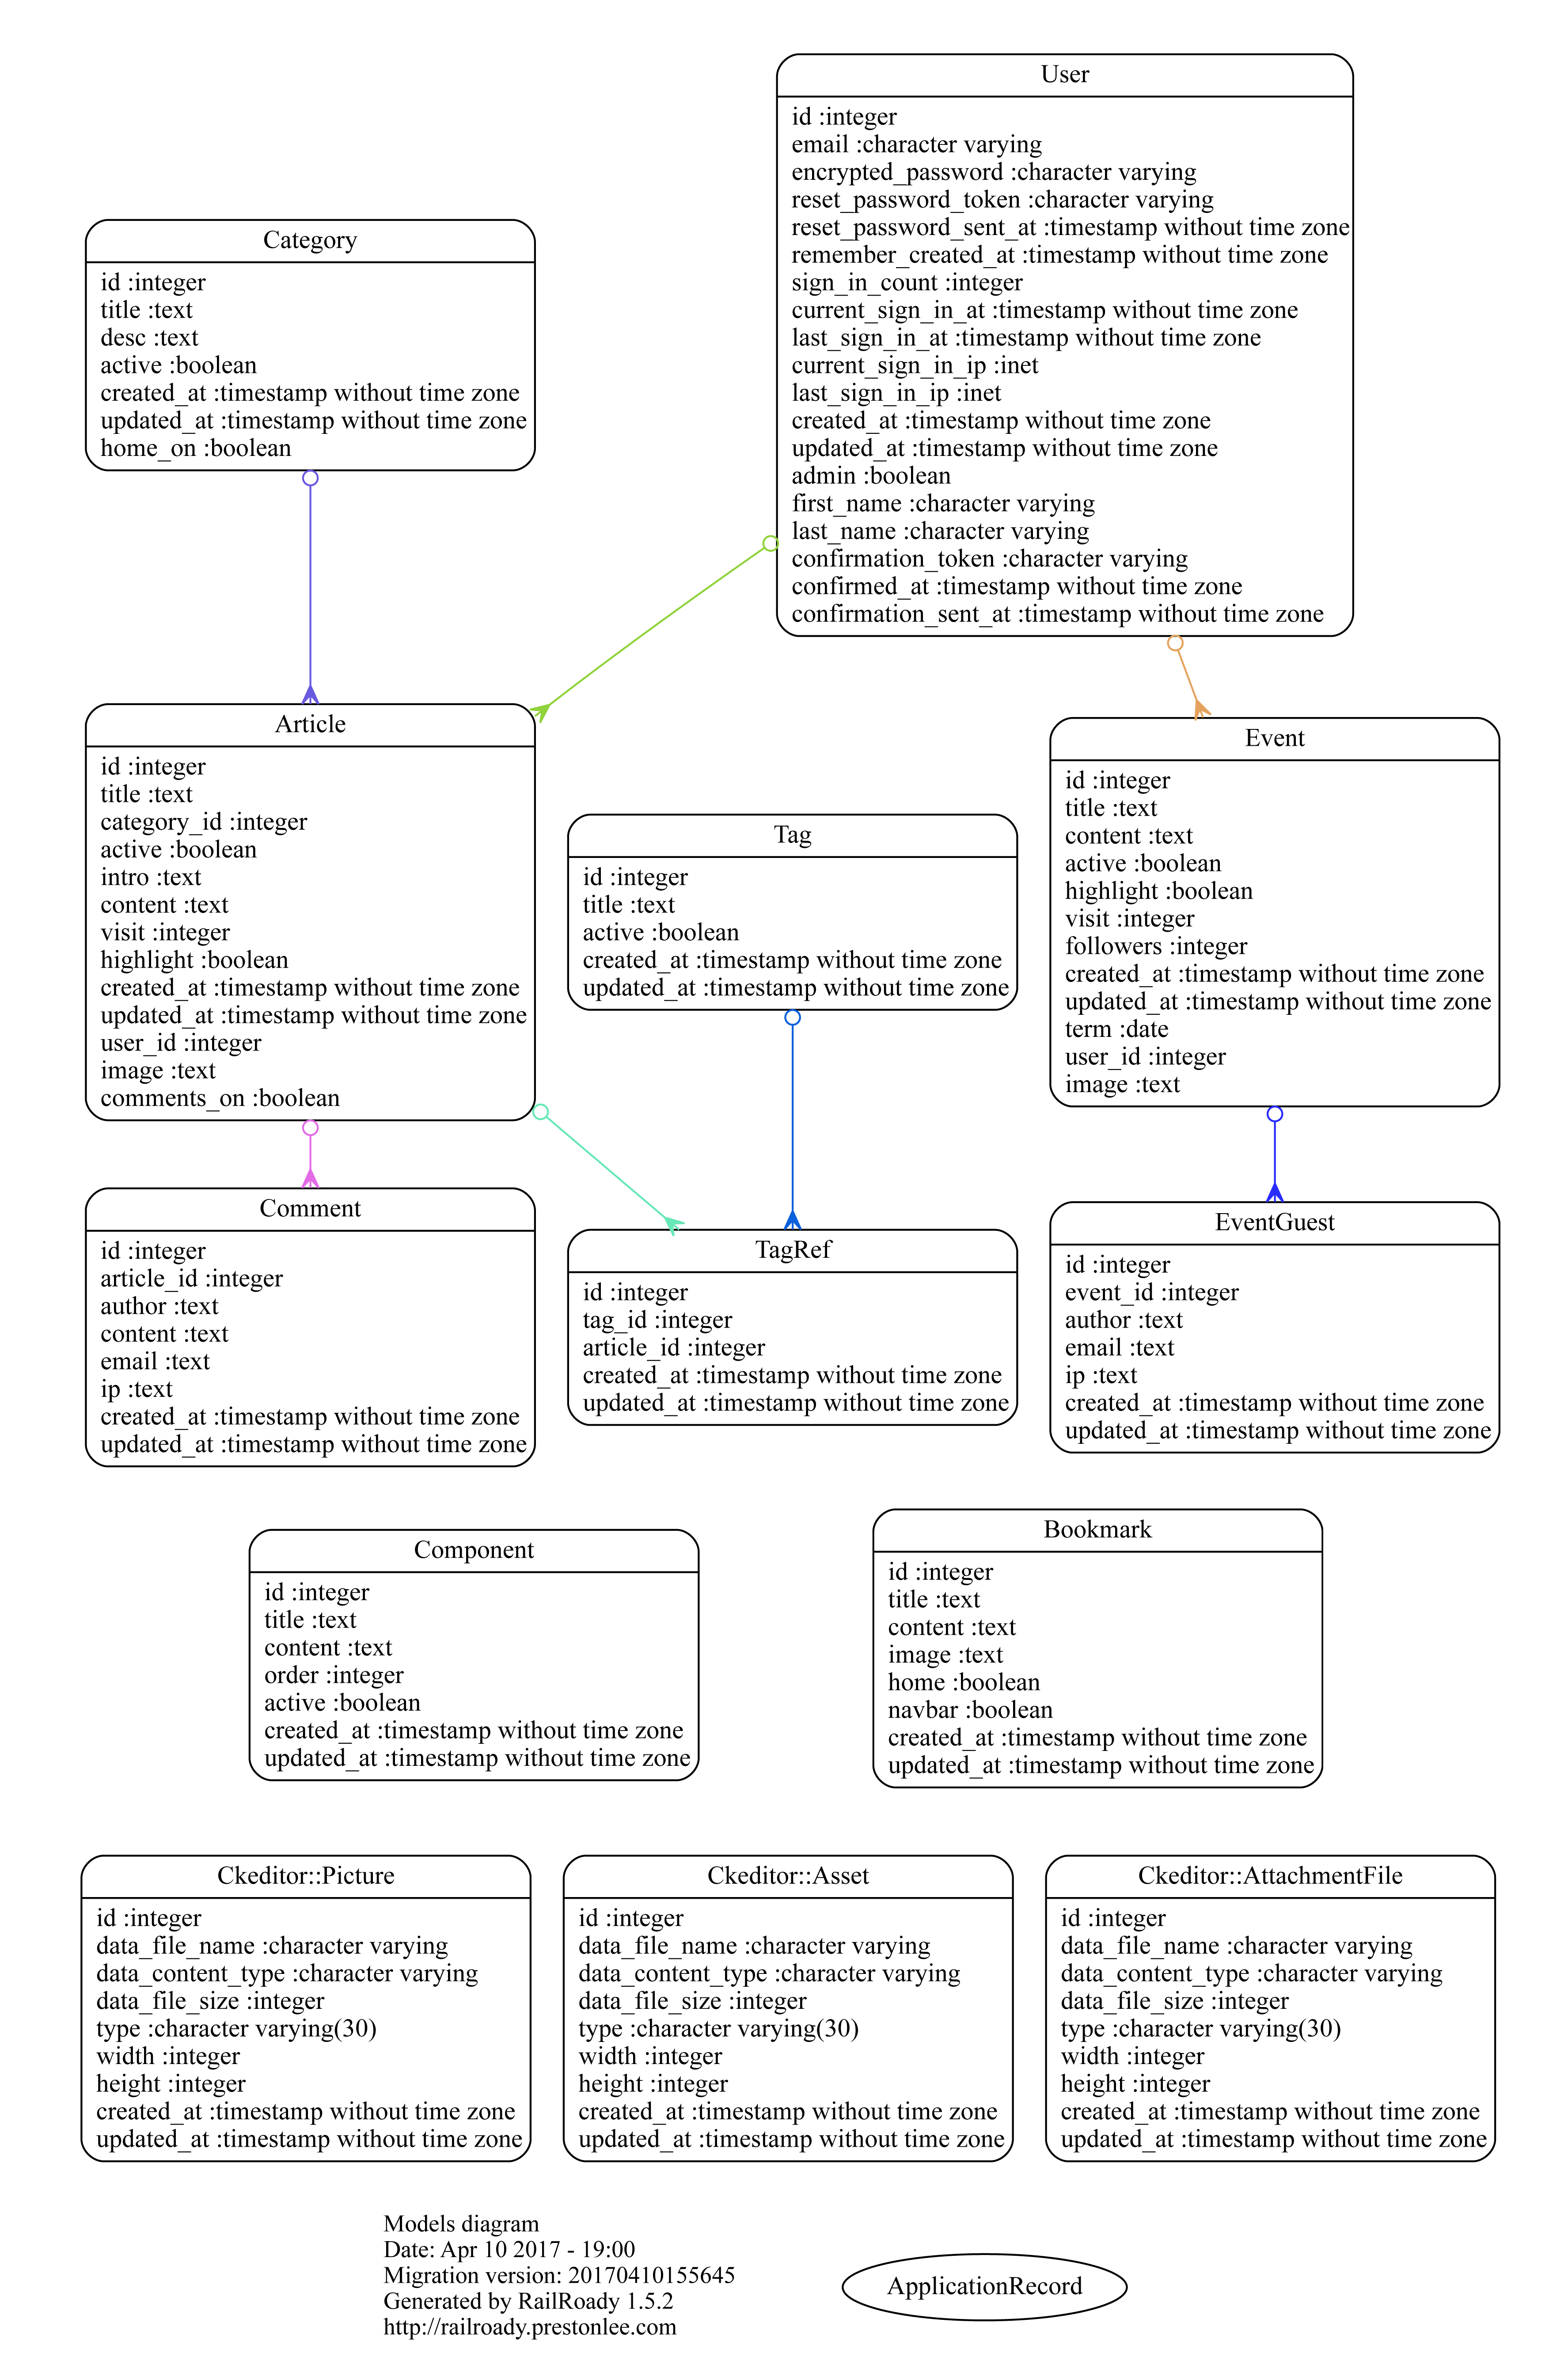
\includegraphics[width=.8\linewidth]{fig/erd2}
\caption{Diagram związków encji\label{RYS.1}}
\source{Opracowanie własne}
\end{figure}

\section{Diagram kontrolera danych}
\begin{figure}[!tbh]
\centering
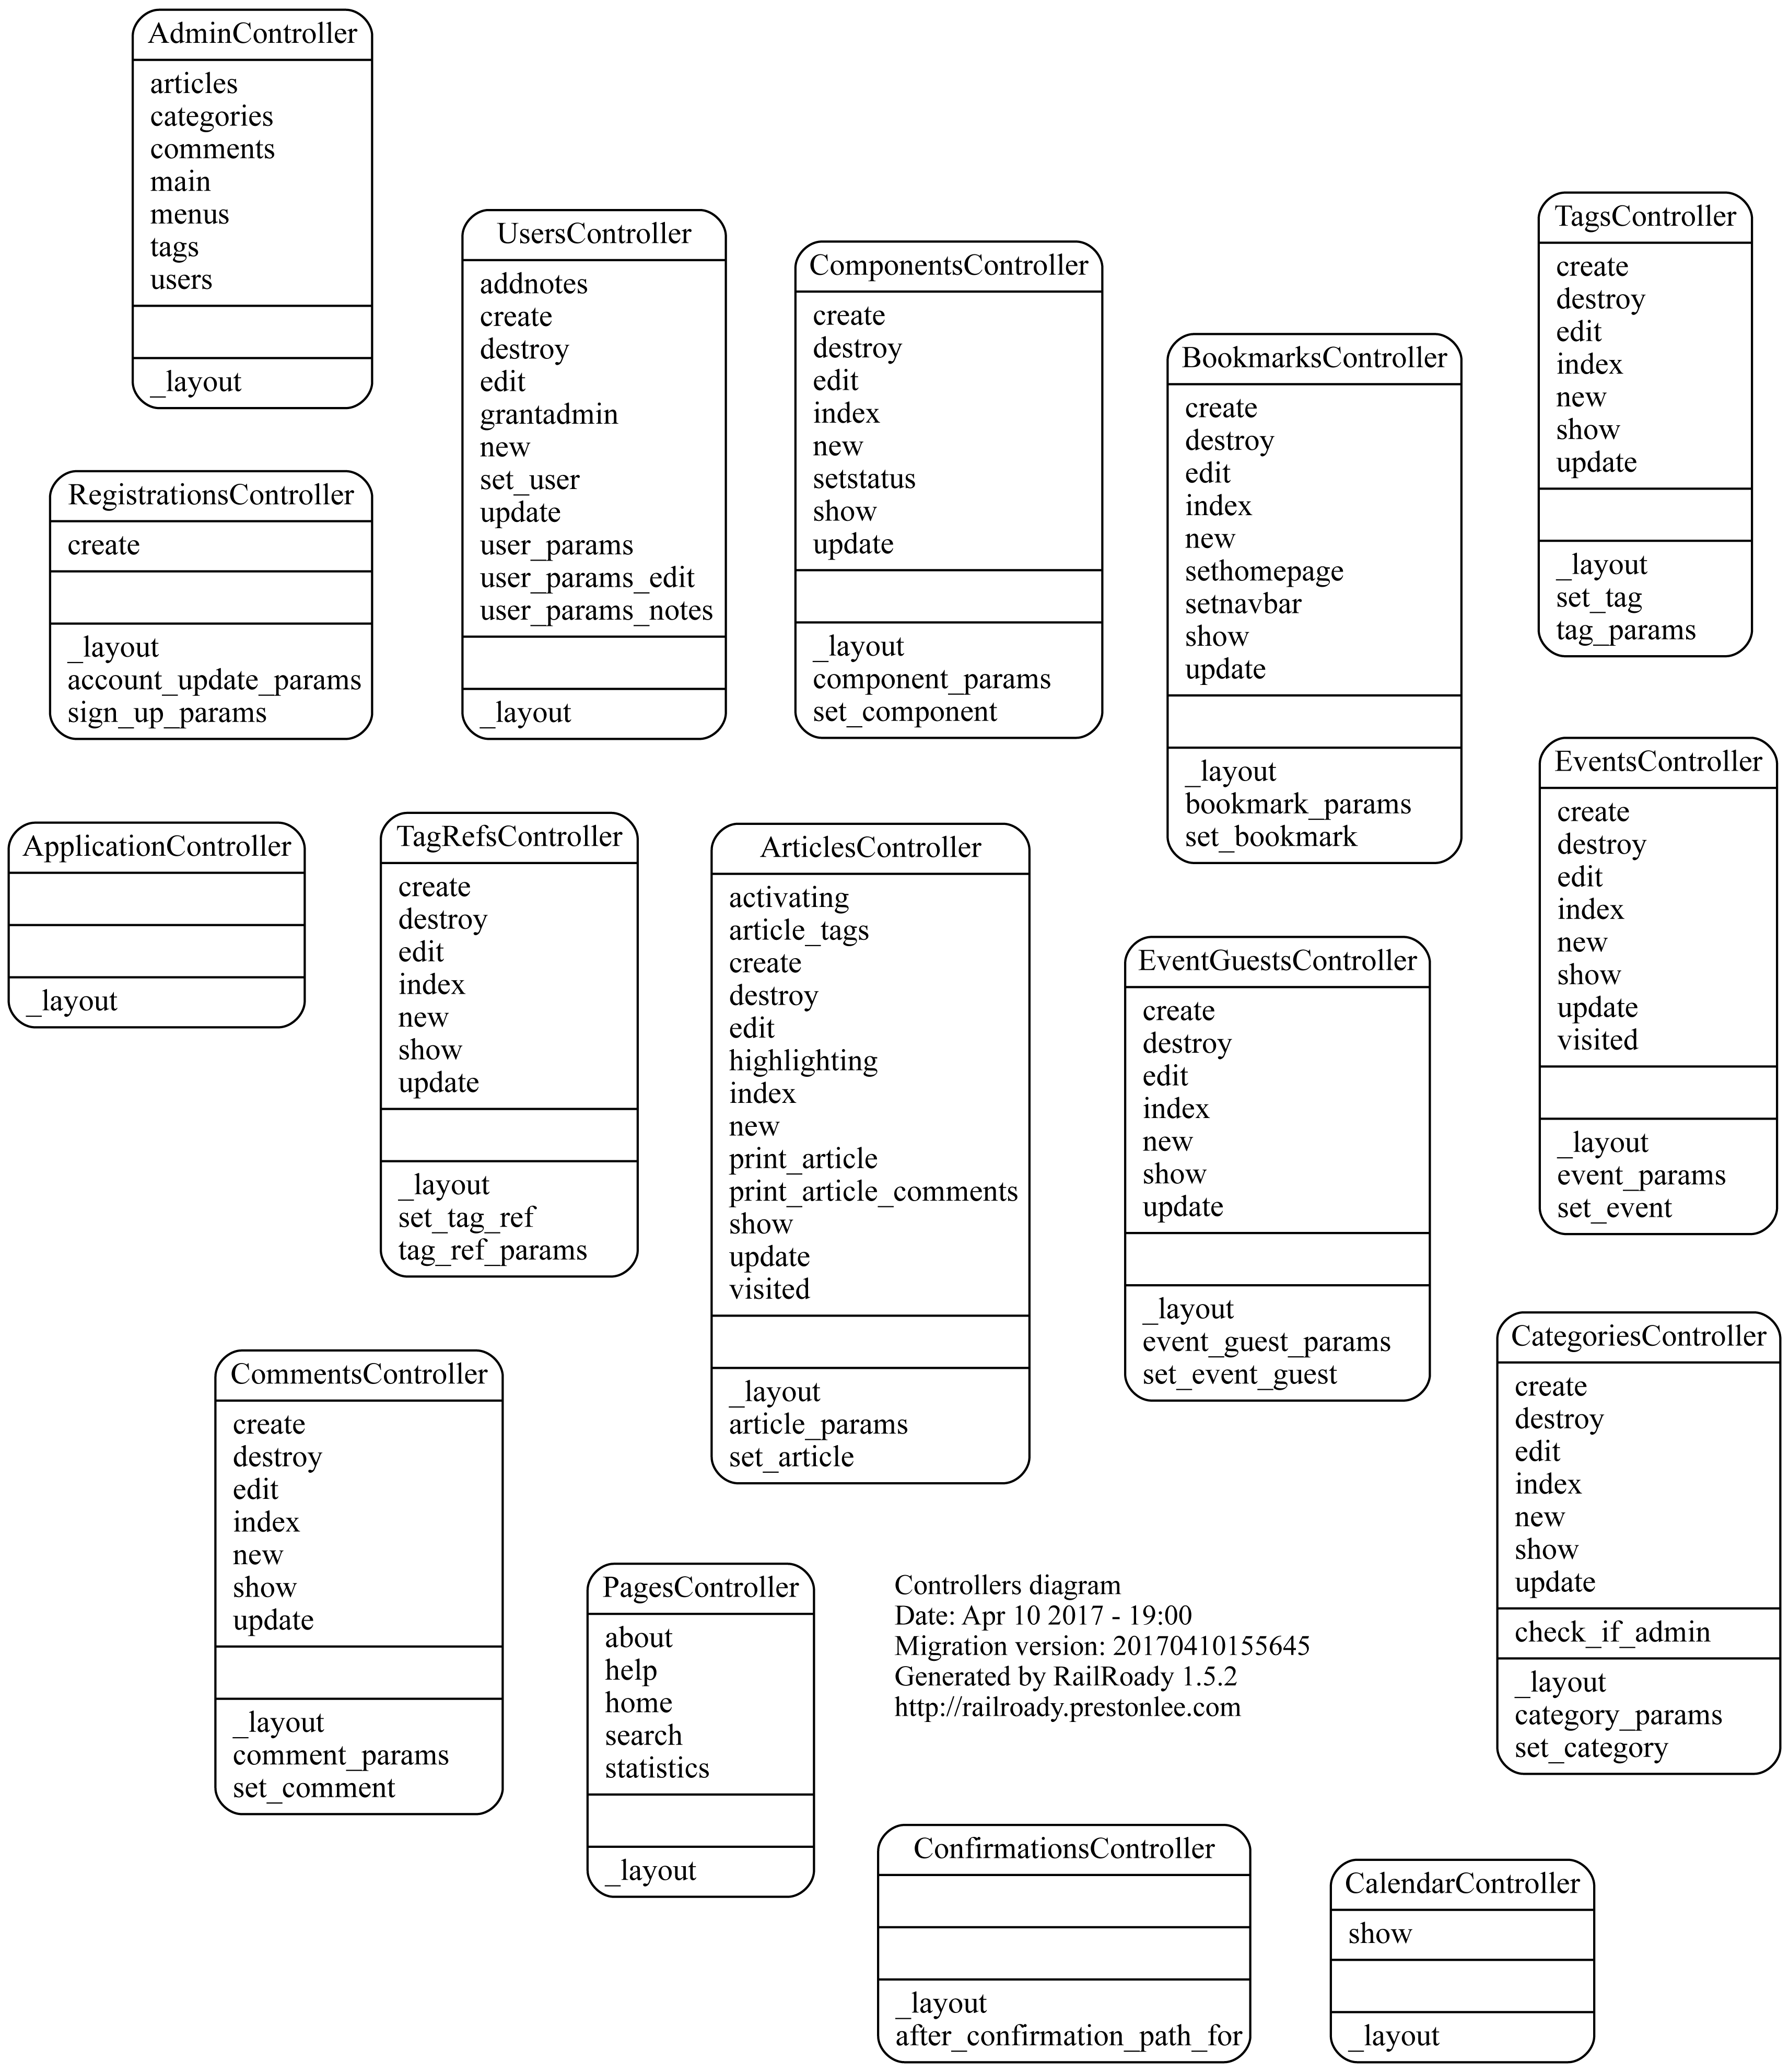
\includegraphics[width=.9\linewidth]{fig/controllers}
\caption{Diagram kontrolera danych\label{RYS.2}}
\source{Opracowanie własne}
\end{figure}

\newpage

\section{Diagram Przypadków Użycia}
\begin{figure}[!tbh]
\centering
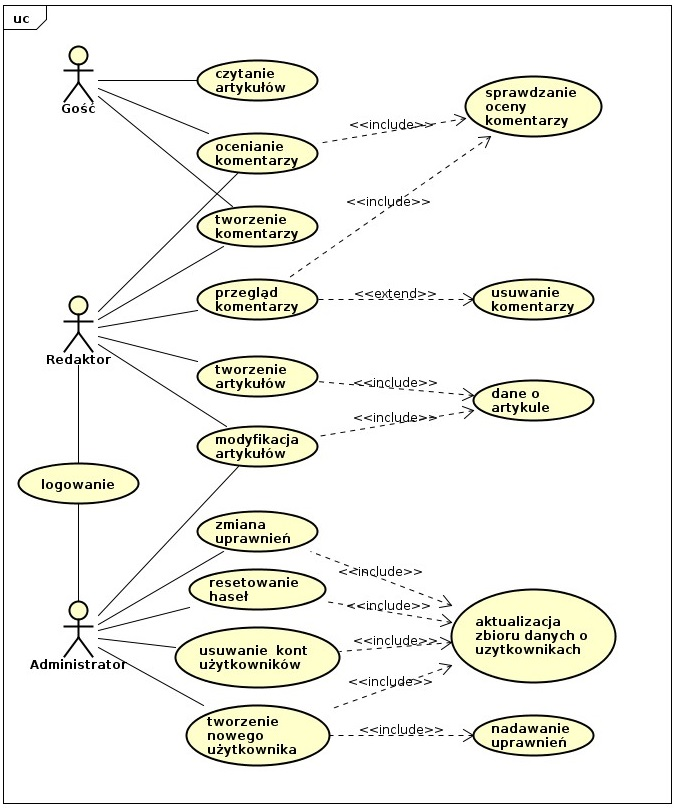
\includegraphics[width=.9\linewidth]{fig/uc}
\caption{Diagram Przypadków Użycia.\label{RYS.6}}
\source{Opracowanie własne}
\end{figure}

\section{Projekt interfejsu użytkownika}

\subsection{Panel Administracyjny}
\begin{figure}[!tbh]
\centering
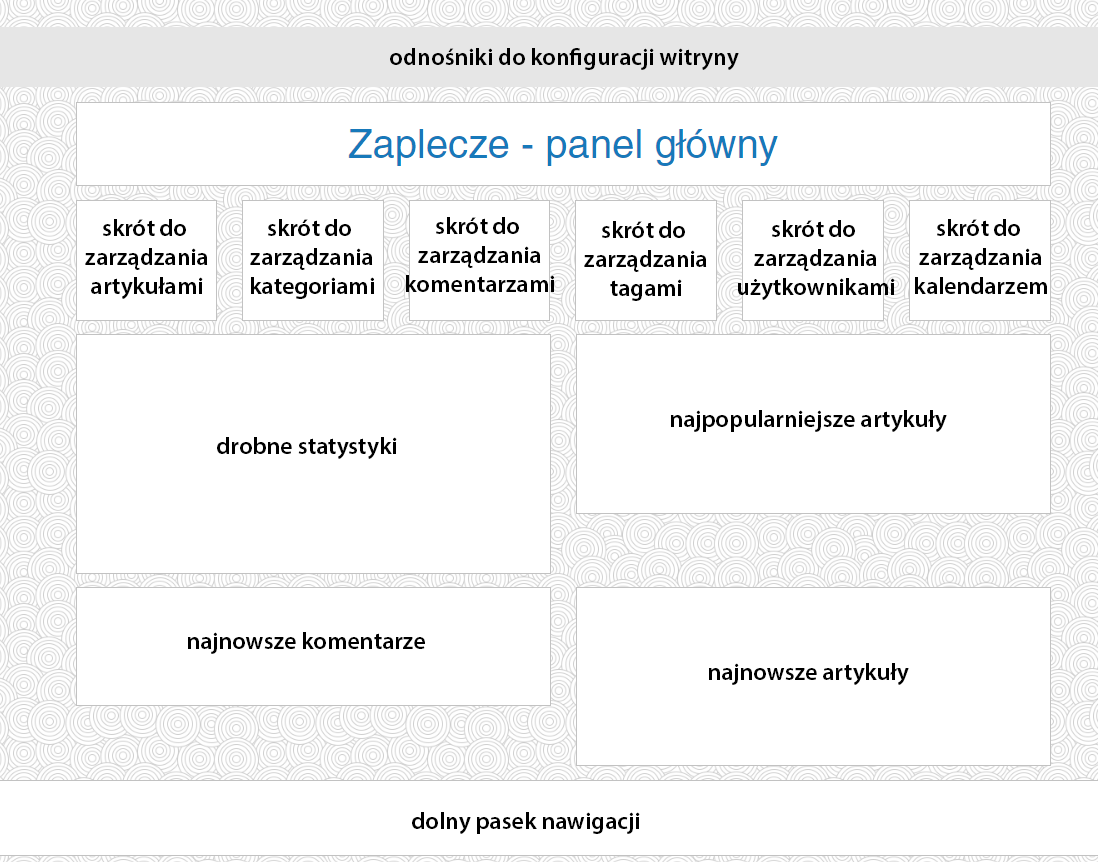
\includegraphics[width=.9\linewidth]{fig/gui_admin}
\caption{Projekt interfejsu użytkownika. Panel Administracyjny.\label{RYS.3}}
\source{Opracowanie własne}
\end{figure}

\newpage

\subsection{Widok Redaktora}
\begin{figure}[!tbh]
\centering
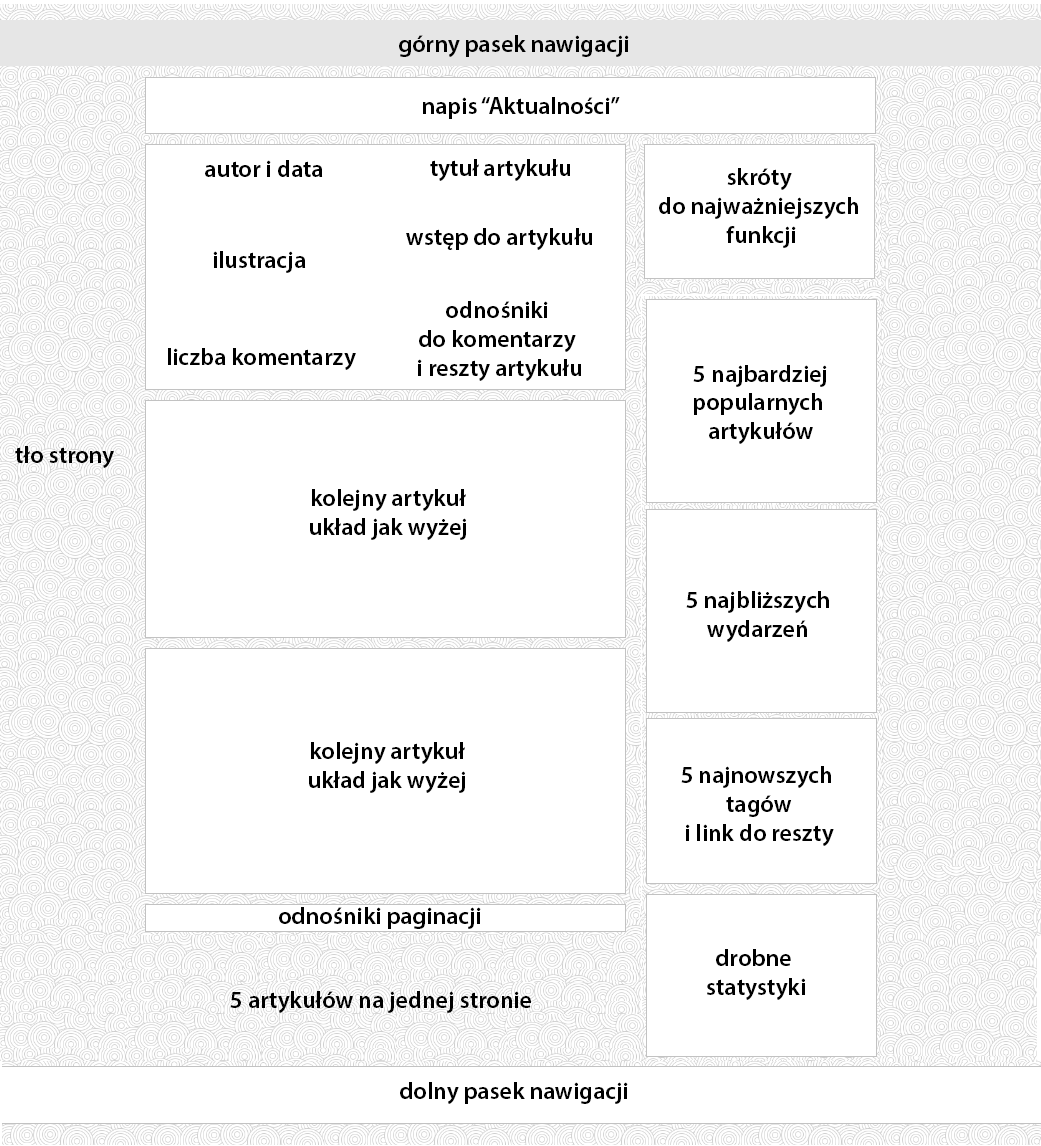
\includegraphics[width=.9\linewidth]{fig/gui_editor}
\caption{Projekt interfejsu użytkownika. Widok Redaktora.\label{RYS.4}}
\source{Opracowanie własne}
\end{figure}

\newpage

\subsection{Widok Gościa}
\begin{figure}[!tbh]
\centering
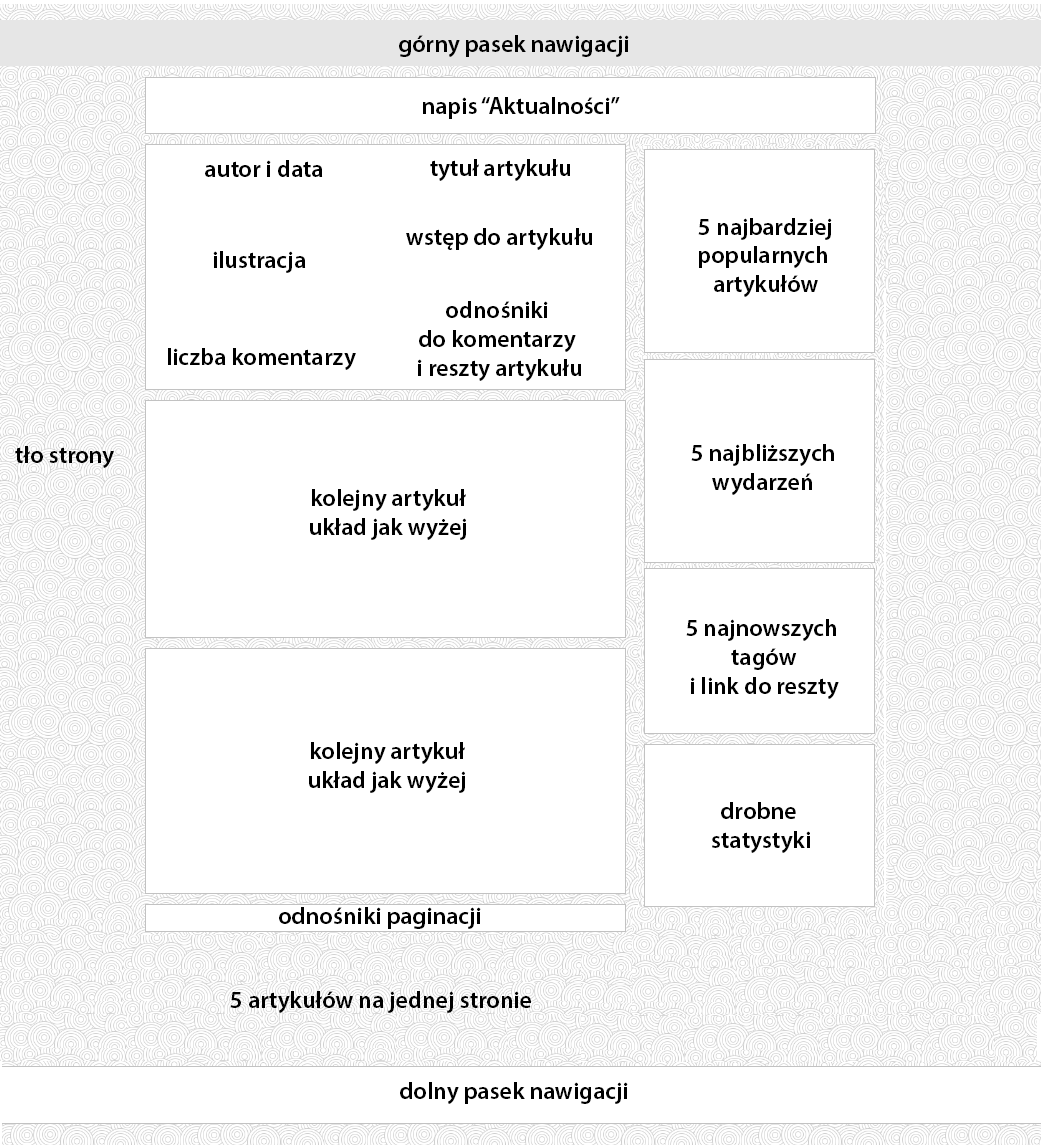
\includegraphics[width=.9\linewidth]{fig/gui_guest}
\caption{Projekt interfejsu użytkownika. Widok Gościa.\label{RYS.5}}
\source{Opracowanie własne}
\end{figure}

\chapter{Implementacja}

\section{Architektura rozwiązania - Ruby on Rails}
Głównym rusztowaniem całego systemu jest framework Ruby On Rails \cite{ror} \cite{enterprise} \cite{wikibook}. Odpowiada on za całość frontendu i backendu. Do swojego działania używa bazy PostgreSQL. W dalszych podrozdziałach przybliżę jak wyglądała implementacja poszczególnych elementów systemu za pomocą Ruby On Rails.

\subsection{Artykuły i Kategorie}
Podstawą jednostką można na stronie jest artykuł, który zawsze zawiera się w którejś z uprzednio utworzonych kategorii. Artykuł posiada atrybuty takie jak tytuł, wstęp, treść główną, numer kategorii do której został przypisany, ilustrację, znacznik aktywności, znacznik wyróżnienia, znacznik komentarzy, liczbę wyświetleń oraz znaczniki czasowe – data i czas utworzenia i edycji. Chciałbym przybliżyć niektóre z atrybutów, pierwszym z nich będą znaczniki aktywności, wyróżnienia i komentarzy, które kolejno oznaczają informacje o tym, że artykuł jest aktywny co przekłada się na to, że będzie wyświetlony na stronie głównej oraz liście artykułów danej kategorii, kolejny atrybut determinuję to, że artykuł zostanie wyświetlony na karuzeli ilustracji na szczycie strony głównej, ostatni ze znaczników pozwala dezaktywować moduł komentarzy, tak jakbyśmy zachcieli, aby przy pewnym artykule nie miałoby być komentarzy. Liczba wyświetleń jest sumaryczną wartością wszystkich odsłon artykułu, polega to na pobraniu liczby wyświetleń z bazy danych następnie zwiększeniu jej o jeden oraz aktualizacji wartości w bazie danych. Znaczniki czasowe są automatycznie dodawane przez Rails. Zarówno na stronie głównej jak i na liście artykułów danej kategorii wyświetlany jest tytuł, wstęp do artykułu, ilustracja, autor, data utworzenia, liczba komentarzy. Po przejściu do artykułu zobaczymy pełną treść, w tym celu właśnie istnieją dwa oddzielne atrybuty. Treść oraz wstęp możemy podczas tworzenia artykułu edytować za pomocą edytora CKEditor, opublikowanego na wolnej licencji. Zaimplementowana został również wyszukiwarka artykułów, które możemy poszukiwać za pomocą treści tytułu. Algorytm ignoruje wielkość liter oraz pozwala szukać za pomocą fragmentów wyrazów. Artykuły mogą dodawać jedynie zalogowaniu użytkownicy. Po przejściu do artykułu możemy go wydrukować dzięki specjalnie do tego przygotowanej formatce optymalizującej miejsce na stronie. 

Kategoria posiada wymienione artykuły: tytuł, opis, znacznik aktywności, znacznik strony głównej oraz znaczniki czasowe – data i czas utworzenia i edycji. Wszystkie kategorie oznaczone jako aktywne wyświetlane są na górnym pasku nawigacji, po przejściu w link danej kategorii zobaczymy opis kategorii oraz listę wszystkich artykułów przypisanych do danej kategorii. Istnieje również taki atrybut jak znacznik strony głównej który określa to czy artykuły przypisane do kategorii będą wyświetlane na stronie głównej. Do strony głównej może być przypisane kilka kategorii. 

\subsection{Komentarze}
Do każdego artykułu możemy dodawać nie długie komentarze. Ta funkcjonalność udostępniona jest dla gości odwiedzających stronę więc co za tym idzie nie jest wymagane logowanie, aby dodać komentarze. W celu dodania komentarza musimy podać swój adres e-mail, który jednak nie jest weryfikowany, jest to powszechnie stosowana praktyka. W bazie danych zapisywany jest także adres IP autora komentarza. Każdy komentarz można ocenić w skali plus/minus. Przy treści komentarza wyświetlana jest wartość oceny, która może być również ujemna. Jeden odwiedzający może ocenić jeden komentarz jeden raz, informacja o tym fakcie zapisywana jest w ciasteczkach.

\subsection{Tagi}
W celu dodatkowej kategoryzacji oraz łatwiejszego znajdowania poszukiwanych przez odwiedzających treści zaimplementowano tagi artykułów. Po utworzeniu artykułu możemy przejść do formularza dodawania tagów, w którym za pomocą listy rozwijanej wybieramy dopasowane tagi, w tym samym miejscu, jeżeli nie znajdziemy poszukiwanych przez nas tagów, możemy dodać swój tag i go przydzielić do artykułu.

\subsection{Kalendarz Wydarzeń}
Zaimplementowany został również kalendarz wydarzeń, który wyświetla dodane wydarzenia w formie klasycznego kalendarza ściennego podzielonego na miesiące. Każde wydarzenie, częściowo na wzór artykułu, posiada atrybuty takie jak tytuł, treść, termin wydarzenia, ilustrację, znacznik aktywności, znacznik wyróżnienia, liczbę wyświetleń oraz znaczniki czasowe – data i czas utworzenia i edycji. Podobnie jak w przypadku artykułów treść możemy podczas tworzenia  edytować za pomocą edytora CKEditor, opublikowanego na wolnej licencji. Znaczniki aktywności i wyróżnienia są odpowiedzialne odpowiednio za wyświetlanie się wydarzenia na kalendarzu oraz na liście po kalendarzem oraz wyświetlanie wydarzeń na karuzeli na szczycie strony głownej. 

Goście odwiedzający stronę mogę się zapisywać do wybranego przez siebie wydarzenia, które polega na podaniu swojego imienia oraz adresu e-mail, ponadto w tle do bazy danych trafia również adres IP osoby się zapisującej. Wydarzenia mogą tworzyć jedynie zalogowaniu użytkownicy.

\subsection{Zakładki}
W celu uporządkowania statycznych informacji prezentowanych na stronie zaimplementowano zakładki. Za pomocą atrybutów przypisanych do danej zakładki możemy określać tytuł, treść, ilustrację, znacznik strony głównej, znacznik paska nawigacji oraz znaczniki czasowe – data i czas utworzenia i edycji. Znacznik strony głównej decyduje o tym, że dana zakładki będzie pełniła rolę właśnie strony głównej. Natomiast znacznik paska nawigacji determinuje fakt wyświetlenia odnośnika do zakładki na górnym pasku nawigacji. Aby zakładka została wyświetlona na stronie głównej konieczne jest zaznaczenie tylko jednej zakładki w przypadku, gdy zostaną więcej niż dwie to strona główna przybierze formę dynamiczną.

\subsection{Strona główna}
Strona główna może zostać skonfigurowana dwojako. Pierwszy sposób polega na wyświetlaniu listy artykułów oraz jej stronicowaniu za pomocą Gema o nazwie \texttt{will\_paginate}. Jak wcześniej wspomniałem na stronie głównej wyświetlone zostaną tylko artykuły aktywne z aktywnych kategorii. Na szczycie głównej witryny pojawi się również karuzela z wyróżnionymi artykułami a i wydarzeniami. Drugim sposobem aranżacji strony głównej jest jest statyczna wersja organizowana za pomocą wyżej opisanych zakładek. Na stronie głównej możemy umieszczać także komponenty, są to ramki z pewną treścią. Na stałe zostały osadzone cztery komponenty zawierające listę popularnych artykułów, listę najbliższych wydarzeń, listę najnowszych tagów oraz drobne statystyki. Komponenty za wzór innych modułów strony posiadają znacznik aktywności, który określa czy dany komponent będzie wyświetlony na stronie głównej. 

\newpage

\section{ZURB Foundation}
ZURB Foundation \cite{foundation} jest responsywnym frameworkiem frontendu. Został stworzony w 2011 roku i dystrybuowany jest na licencji MIT License. W systemie \mbox{TrainCMS} odpowiada za frontend. 

\subsection{Instalacja}
Dołączenie Foundation do projektu Ruby On Rails polega na zainstalowaniu Gema o nazwie \texttt{foundation-rails}. Następnie przeprowadzeniu automatycznej instalacji za pomocą polecenia 
\begin{lstlisting}[language=bash, caption={Polecenie instalujące Foundation w naszym projekcie}]
$ rails g foundation:install 
\end{lstlisting} 
oraz dodaniu odpowiednich zapisów w plikach kaskadowych arkuszy stylów i plikach skryptów JavaScript.

\subsection{Użycie}
Podczas budowy całego systemu zarządzania treścią strony internetowej korzystałem z bogatej biblioteki komponentów jaką oferuje framework Foundation. Każda zaimplementowana tabela otrzymała klasę 
\begin{lstlisting}[language=html, caption={Przykładowa tabela}]
<table class="stack"></table>
\end{lstlisting}
która odpowiedzialna jest za wyświetlanie tabeli w mobilnym widoku jako stos kolumn, wiersze tabeli wyświetlane są na przemian kolor biały z kolorem grafitowym, tę funkcję również  zawdzięczamy Foundation. Wszystkie odnośniki \mbox{posiadają klasę}
\begin{lstlisting}[language=html, caption={Przykladowy przycisk}]
<%= link_to 'odnosnik', odnosnik_path, 
	class:'button' %>
\end{lstlisting}
co pozwala na wyświetlania każdego odnośnika w formie prostokątnego z ostrymi rogami przycisku. Jednakże wszystkie odnośniki nie są przyciskami o tej samej wielkości, odnośniki zawarte w tabeli mają dodatkową klasę 
\begin{lstlisting}[language=html, caption={Przykładowy przycisk}]
<%= link_to 'maly odnosnik', maly_odnosnik_path, 
	class:'tiny button' %>
\end{lstlisting}
dzięki której przycisk staję bardzo mały i w elegancki sposób wkomponowuje się w wiersze tabeli. Również do nawigacji po stronicowaniu wykorzystano metodę renderowania w stylu Foundation. Ogólna konwencja graficzna opiera się na siatce, opisanej za pomocą znaczników \texttt{div}. Każda sekcja wszystkich stron poszczególnych modułów całego systemu zapisana jest w znaczniku \texttt{div}, który otrzymuje za każdym razem klasę 
\begin{lstlisting}[language=html, caption={Przykładowy div}]
<div class="callout"></div>
\end{lstlisting}
która powoduje wyświetlanie treści na białym eleganckim prostokącie z ostrymi rogami. Strona główna została podzielona za pomocą siatki znaczników \texttt{div} na kilka sekcji. Formularze wprowadzania danych wykorzystują klasę \texttt{div} 
\begin{lstlisting}[language=html, caption={Przykładowe pole tekstowe}]
<div class="input-group">
	<span class="input-group-label">Tytul</span>
         <%= f.text_field :title, type:"text", 
		class:"input-group-field" %>
</div>
\end{lstlisting}
która pozwala na wyświetlanie etykiety pola i samego w jednej linii oszczędzając miejsce i prezentując stronę jeszcze bardziej czytelniejszą. 

\newpage

\section{CarrierWave, CKEditor, Cloudinary}
\subsection{CarrierWave i Cloudinary}
CarrierWave \cite{carrierwave} jest to Gem usprawniający obsługę plików różnych rozszerzeń dla aplikacji w Rubym, natomiast Cloudinary jest to usługa oferująca na umieszczanie plików na bezpłatnym serwerze hostingowym, dodatkowo o tej samej nazwie istnieje Gem, który obsługują całą tę funkcjonalność z poziomu aplikacji Ruby. Oba rozwiązania są ze ściśle sobą powiązane, ale mogą też działać samodzielnie. Gemy udostępnione są na licencji MIT License. 

Gem należy dodać do pliku gemfile. Następnie utworzyć uploader za pomocą polecenia: 
\begin{lstlisting}[language=bash]
rails generate uploader Avatar
\end{lstlisting}
które wygeneruje plik, w którym to możemy przeprowadzić konfigurację. Dodatkowo do swojego pełnego działania potrzebuje pakiet RMagick, który możemy zainstalować za pomocą polecenia: 
\begin{lstlisting}[language=bash, caption={Polecenie instalujące oprogramowanie RMagick}]
sudo apt-get install imagemagick libmagickwand-dev
\end{lstlisting}
Przed przejściem do dalszych kroków należy mieć założone konto w serwisie Clodinary, z tego też serwisu po zalogowaniu pobieramy plik konfiguracyjny przygotowany dla aplikacji napisanych w Ruby, zapisujemy go w katalogu \texttt{/config}. Do każdego z plików uploadera, których należy dodać dwie linie 
\begin{lstlisting}[language=ruby, caption={Framgent zawartości pliku uploadera}]
include CarrierWave::Rmagick
include Cloudinary::CarrierWave.
\end{lstlisting}

\newpage

W celu zachowania porządku na serwerze usługi Cloudinary w każdym pliku możemy dodać linię oznaczjacą tagiem każdy załadowany przez nas plik: 
\begin{lstlisting}[language=ruby, caption={Przykładowy tag dla pliku}]
process :tags => ['random_tag']
\end{lstlisting}
Aby wyświetlić załadowany plik, na przykład obraz należy dodać linię o treści: 
\begin{lstlisting}[language=html, caption={Kod wyświetlający obraz}]
<%= image_tag @article.image.url %>
\end{lstlisting}

\subsection{CKEditor}
CKEditor \cite{ckeditor} jest edytorem WYSIWYG\footnote{\textit{ang. what you see is what you get} skórt oznaczjący "to co widzisz, to otrzymasz", stosowany w technikach komputerowych do określenia rozwiązań pozwalających uzyskać już podczas produkcji tekstu wynik wielce zbliżony lub niemalże identyczny do finalnego efektu.}, który umożliwią łatwą i przyjemna edycje tekstu w oknie przeglądarki możliwościami zbliżonymi do edytora tekstu klasy Microsoft Word. Gem udostępniony jest na licencji MIT License. 

W celu instalacji należy dodać gem do pliku gemfile. W drugim kroku dodać do pliku \texttt{config/initializers/ckeditor.rb} linie: 
\begin{lstlisting}[language=ruby, caption={Framgent zawartości pliku ckeditor.rb}]
Ckeditor.setup do |config|
  config.cdn_url = 
	"//cdn.ckeditor.com/4.6.1/basic/ckeditor.js"
end
\end{lstlisting}

\newpage

Następnie w pliku \texttt{/app/views/layouts/application.html.erb} linię o następującej treści:
\begin{lstlisting}[language=html, caption={Framgent zawartości pliku application.html.rb}]
<%= javascript_include_tag "chartkick" %>
\end{lstlisting}
W miejscu, w którym chcemy użyć ten komponent dodajemy linię o treści:
\begin{lstlisting}[language=html, caption={Kod uruchamiajacy edytor}]
<%= f.cktext_area :content, placeholder:"Content" %>
\end{lstlisting}
Rozwiązanie to ściśle współpracuje z przedstawionym wyżej rozwiązaniem publikacji załączników, na przykładzie artykułów, możemy nie tylko dodać główną ilustrację publikacji, ale także za pomocą CKEditora dodać kilka innych załączników, nie tylko obrazków, które także znajdą się na serwerze usługi Cloudinary. 

\newpage

\section{Prawn}
Prawn \cite{prawn} jest gemem generującym pliki w formacie PDF. Udostępniano został na licencji GPL.

Aby zainstalować gem w naszym projekcie, należy go dodać do pliku Gemfile. W celu utworzenia plików PDF należy utworzyć klasę w kontrolerze, która będzie dziedziczyła z klas gemu:
\begin{lstlisting}[language=ruby, caption={Deklaracja klasy generującej plik PDF}]
class ArticleOnePdf < Prawn::Document
\end{lstlisting}
Wykorzystanie Prawn umożliwia bardzo precyzyjne, pod względem rozmieszczania poszczególnych elementów, projektowanie dokumentów. Do generowanych dokumentów możemy dodawać obrazy, tabelę  i wiele innych elementów. Podczas generowania precyzujemy rozmiar oraz orientację strony. 
\begin{lstlisting}[language=ruby, caption={Kod generujacy dokment zawierający ilustrację i wstęp do artykułu}]
class ArticleOnePdf < Prawn::Document
  def initialize(article)
    super()
    @article = article    

    move_down 10
    photo = "#{Rails.root}/public#{@article.image.url}"
    image photo, :width => 400

    move_down 10
    font("SourceSansPro-Bold.ttf", size: 14) do
      text "#{remove_html(@article.intro)}"
  end
end
\end{lstlisting}

\newpage

\section{Chartkick}
Chartkick \cite{chartkick} jest gemem, który z pewnością wzbogaci wizualnie każdy projekt w którym się znajdzie. Głównym zadaniem gema jest generowanie wykresów. Pierwszy raz został opublikowany w 2013 i teraz udostępniany jest na licencji \mbox{MIT License. }

W celu zainstalowania gema należy dodać go do pliku Gemfile, następnie w pliku \texttt{application.js} dodać linię 
\begin{lstlisting}[language=html, caption={Framgent zawartości pliku application.js}]
//= require chartkick
\end{lstlisting}
natomiast w pliku \texttt{layouts/application.html.erb} dodać linię:
\begin{lstlisting}[language=html, caption={Framgent zawartości pliku application.html.rb}]
<%= javascript_include_tag "//www.google.com/jsapi", 
"chartkick" %>
\end{lstlisting}

\newpage

Bardzo ciekawym wykresem jest wykres o nazwie \texttt{pie\_chart}. Można go umieścić w następujący sposób:
\begin{lstlisting}[language=html, caption={Kod uruchamiający wykres kołowy}]
<%= pie_chart Article.group(:title).sum(:visit) %>
\end{lstlisting}
Generuje on bardzo przejrzysty obrazek z wykresem:
\begin{figure}[!tbh]
\centering
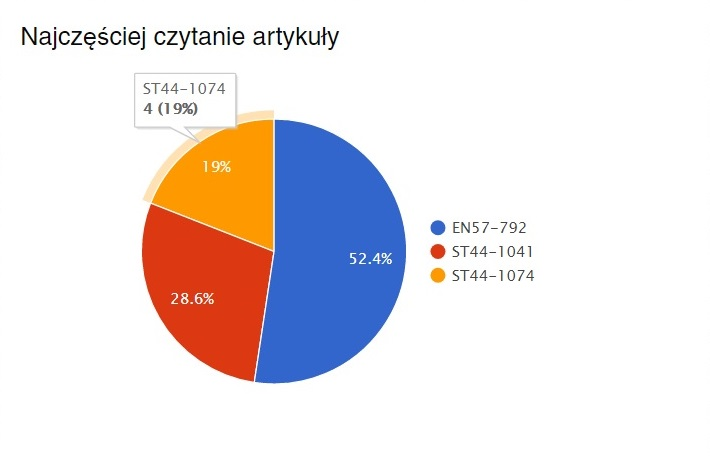
\includegraphics[width=.5\linewidth]{fig/chartkick}
\caption{Wykres kołowy.\label{RYS.6}}
\source{Opracowanie własne}
\end{figure}

\begin{thebibliography}{9}
\bibitem{ror} 
John Elder.
\textit{Learn Ruby On Rails For Web Development: Learn Rails The Fast And Easy Way!}. 
Codemy.com; 1 edition (January 19, 2015).
 
\bibitem{enterprise} 
Dan Chak.
\textit{Enterprise Rails}. 
O'Reilly Media; 1 edition (November 3, 2008).

\bibitem{wikibook} 
Użytkownicy Wikibooks.
\textit{Ruby}. 
Wikibooks; 1 edition (February 17, 2008).

\bibitem{guides} 
Ruby on Rails. Dokumentacja.
\\\texttt{\url{http://guides.rubyonrails.org/}}

\bibitem{api} 
Ruby on Rails API. Dokumentacja.
\\\texttt{\url{http://api.rubyonrails.org/}}

\bibitem{foundation} 
Foundation for Sites. Dokumentacja.
\\\texttt{\url{http://foundation.zurb.com/sites/docs/}}

\bibitem{carrierwave} 
CarrierWave. Dokumentacja.
\\\texttt{\url{https://github.com/carrierwaveuploader/carrierwave/wiki}}

\bibitem{ckeditor} 
CKEditor for Rails. Dokumentacja.
\\\texttt{\url{https://github.com/galetahub/ckeditor/}}

\bibitem{prawn} 
PrawnPDF. Dokumentacja.
\\\texttt{\url{http://prawnpdf.org/api-docs/2.0/}}

\bibitem{chartkick} 
Chartkick. Dokumentacja.
\\\texttt{\url{https://github.com/ankane/chartkick/}}
\end{thebibliography}


% zakończenie
\summary
to do

% załączniki (opcjonalnie):
\appendix
\chapter{Tytuł załącznika jeden}

Treść załącznika jeden.

\chapter{Tytuł załącznika dwa}

Treść załącznika dwa.

% spis rysunków (jeżeli jest potrzebny):
\listoffigures

\lstlistoflistings
\addcontentsline{toc}{chapter}{Spis kodów źródłowych}%

\oswiadczenie

\end{document}
